\documentclass{article}
\usepackage{amsmath}
\usepackage{amssymb}
\usepackage{graphicx}
%\usepackage{enumitem}
\usepackage[utf8]{inputenc}
\graphicspath{{../Imagenes/}}

\title{\Huge Taller de Herramientas Computacionales}
\author{Elías Jiménez Cruz}
\date{15/enero/2019}

\begin{document}
	\maketitle
	\begin{center}
		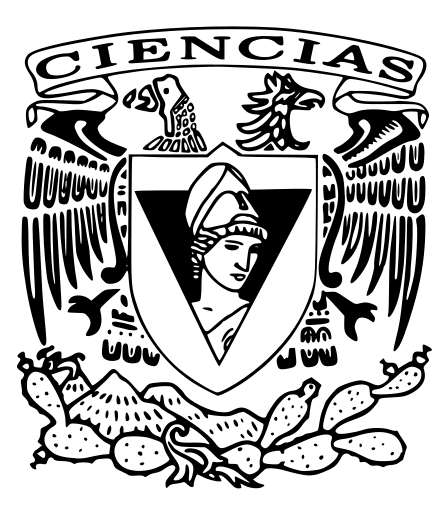
\includegraphics[scale=0.40]{EscudoFC.png}
	\end{center}
	\newpage
	\section*{Expresiones Matemáticas} %Sin asterisco se enumeran las secciones
	$\alpha + \beta$ \\
	\(\alpha +\beta\) \\
	\[\alpha + \beta\]
	\section*{Índices y subíndices}
	$x {2}$
	$x^{2}$
	\section*{Fracciones}
	$\frac{\frac{3}{5}}{2}$, 
	$\sqrt{2} + \sqrt{3^2}^2$, 
	\%, %Para mostrar el porcentaje.
	$\int_{a}^{b} x^2 dx$, 
	$\int_{a}^{b} x^2 \partial x^2$\\
	\begin{equation}
		\label{key}
	\end{equation}
	$3 \quad 2$
	\section*{Matrices}
	%\dots puntos suspensivos
	%\vdots puntos suspensivos verticales
	\[
	\begin{bmatrix}
		x_{2} & x_{3}\\
		x_{4} & x_{6}
	\end{bmatrix}
	\]
	\[
	\begin{bmatrix}
	x_{2} & x_{5} & \dots\\
	x_{5} & x_{20} & \dots\\
	\vdots & \vdots & \vdots
	\end{bmatrix}
	\]
	$\sum$
	\section*{Tablas}
	\[
	\begin{array}{|c|c|c|}
	\hline
	f(t) & F(s) & \mbox{remark}\\
	\hline\hline
	\delta(t) & 1 & \mbox{impulse function}\\
	u(t) & \frac{1}{5} & \mbox{unit step function}\\
	e^{at}u(t) & \frac{1}{s-a} & \mbox{one-side exponential }\\
	\hline
	\end{array}
	\]
	\section*{Alineamiento}
	\begin{align*}
	2x - 5y &= 8\\
	2x - 9y &= -12\\
	\end{align*}
	
\end{document}